\documentclass[tikz]{standalone}\input{pre.tex}\begin{document}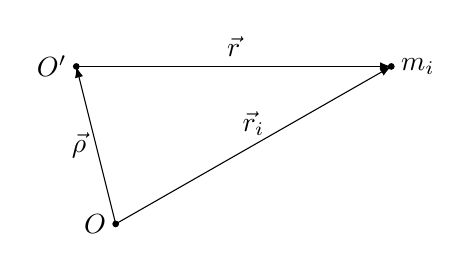
\begin{tikzpicture}
		\coordinate (A) at (0,0);
		\coordinate (B) at (0.5,-2);
		\coordinate (C) at (4,0);
		\draw[fill=black] (C) circle (1pt) node [right] {$m_i$};
		\draw[fill=black] (0,0) circle (1pt) node[left] {$O'$}; 
		\draw[fill=black] (0.5,-2) circle (1pt) node[left] {$O$}; 

		\draw[->, >=latex] (A) -- node [above] {$\vec{r}\zi$} (C);
		\draw[->, >=latex] (B) -- node [above] {$\vec{r}_i$}  (C);
		\draw[->, >=latex] (B) -- node [left] {$\vec{\rho}$}  (A);
	
\end{tikzpicture}\end{document}